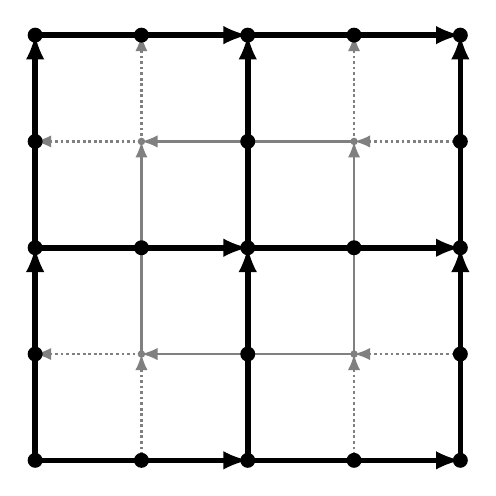
\begin{tikzpicture}[>=latex, line width=2pt, scale=2.7]
\usetikzlibrary{calc}

\edef\n{2}

\pgfmathparse{\n-1}
\edef\nmone{\pgfmathresult}

\pgfmathparse{\n-2}
\edef\nmtwo{\pgfmathresult}

%all the gray (dual) stuff
\begin{scope}[gray,  line width=1pt]
%dual vertices
\foreach \x in {0,...,\nmone} {
	\foreach \y in {0,...,\nmone} {
		\coordinate (V) at (\x+0.5,\y+0.5);
		\fill (V) circle(0.5pt);
	}
}

%dual x-edges
\foreach \x in {0,...,\nmtwo} {
	\foreach \y in {0,...,\nmone} {
		\coordinate (V1) at (\x+0.5,\y+0.5);
		\coordinate (V2) at (\x+1.5,\y+0.5); 
		\draw[<-] (V1) -- (V2);
	}
}

%dual y-edges
\foreach \x in {0,...,\nmone} {
	\foreach \y in {0,...,\nmtwo} {
		\coordinate (V1) at (\x+0.5,\y+0.5);
		\coordinate (V2) at (\x+0.5,\y+1.5); 
		\draw[->] (V1) -- (V2);
	}
}

%all remaining (half) dual edges on the boundaries 
\foreach \xy in {0,...,\nmone} {
	\draw[->,densely dotted] (\xy+0.5, 0) --  (\xy+0.5, 0.5); 
	\draw[->,densely dotted] (\xy+0.5, \n-0.5) --  (\xy+0.5, \n);
	\draw[<-,densely dotted] (0,\xy+0.5) -- (0.5,\xy+0.5);
	\draw[<-,densely dotted] (\n-0.5,\xy+0.5) -- (\n,\xy+0.5);
}
\end{scope}

%primal vertices
\foreach \x in {0,...,\n} {
	\foreach \y in {0,...,\n} {
		\coordinate (V) at (\x,\y);
		\fill (V) circle(1pt);
	}
}

%primal x-edges
\foreach \x in {0,...,\nmone} {
	\foreach \y in {0,...,\n} {
		\coordinate (V1) at (\x,\y);
		\coordinate (V2) at (\x+1,\y); 
		\draw[->] (V1) -- (V2);
	}
}

%primal y-edges
\foreach \x in {0,...,\n} {
	\foreach \y in {0,...,\nmone} {
		\coordinate (V1) at (\x,\y);
		\coordinate (V2) at (\x,\y+1); 
		\draw[->] (V1) -- (V2);
	}
}

%primal edge circumcenters
\foreach \xy in {0,...,\n} {
	\foreach \yx in {0,...,\nmone} {
		\coordinate (VX) at (\yx+0.5,\xy);
		\coordinate (VY) at (\xy,\yx+0.5);
		\fill (VX) circle(1pt);
		\fill (VY) circle(1pt);
	}
}

%%nodes
%\node[below right] at (1,1) {$v_{i,j}$};
%\node[below right] at (2,1) {$v_{i+1,j}$};
%
%\node[above right] at (1.5,1) {$e^x_{i,j}$};
%\node[above right] at (1.5,0) {$e^x_{i,j-1}$};
%\node[above right] at (1.5,2) {$e^x_{i,j+1}$};
%
%\node[below right] at (1,1.5) {$e^y_{i,j}$};
%\node[below right] at (2,1.5) {$e^y_{i+1,j}$};
%\node[below right] at (1,0.5) {$e^y_{i,j-1}$};
%\node[below right] at (2,0.5) {$e^y_{i+1,j-1}$};



\end{tikzpicture}
